\documentclass[12pt]{article}
\usepackage{parskip}
\usepackage{caption}
\usepackage{lipsum}
\usepackage{pgfplots}

\captionsetup{position=top,labelfont=bf, labelsep=space, justification=justified, singlelinecheck=false, skip=1.5pt}
\usepackage{microtype}
\usepackage{booktabs}

\title{Article Template}
\author{Nihal Sahu \and John Doe\thanks{\lipsum[4]}}
\date{\today}
\begin{document}
\maketitle
\begin{abstract}
    \lipsum[5]
\end{abstract}
\newpage
\tableofcontents
\newpage

\section{Introduction}
\lipsum

\begin{table}[htbp]

\hrule height 1pt\medskip
\caption{Ideas and sources}
\hrule
\bigskip
\footnotesize\lipsum[4]
\bigskip
\begin{center}
    \begin{tabular}{ l l l l l }
    \midrule
    Idea & Source \\\midrule
    Typesetting & CV Radhakrishnan \\
    Software Design & Rich Hickey \\
    \end{tabular}
\end{center}
\medskip
\hrule
\end{table}

\begin{figure}
\hrule height 1pt\medskip
\caption{India GDP growth (annual \%)}
\hrule
\bigskip
\footnotesize\lipsum[4]
\bigskip
\begin{center}
 
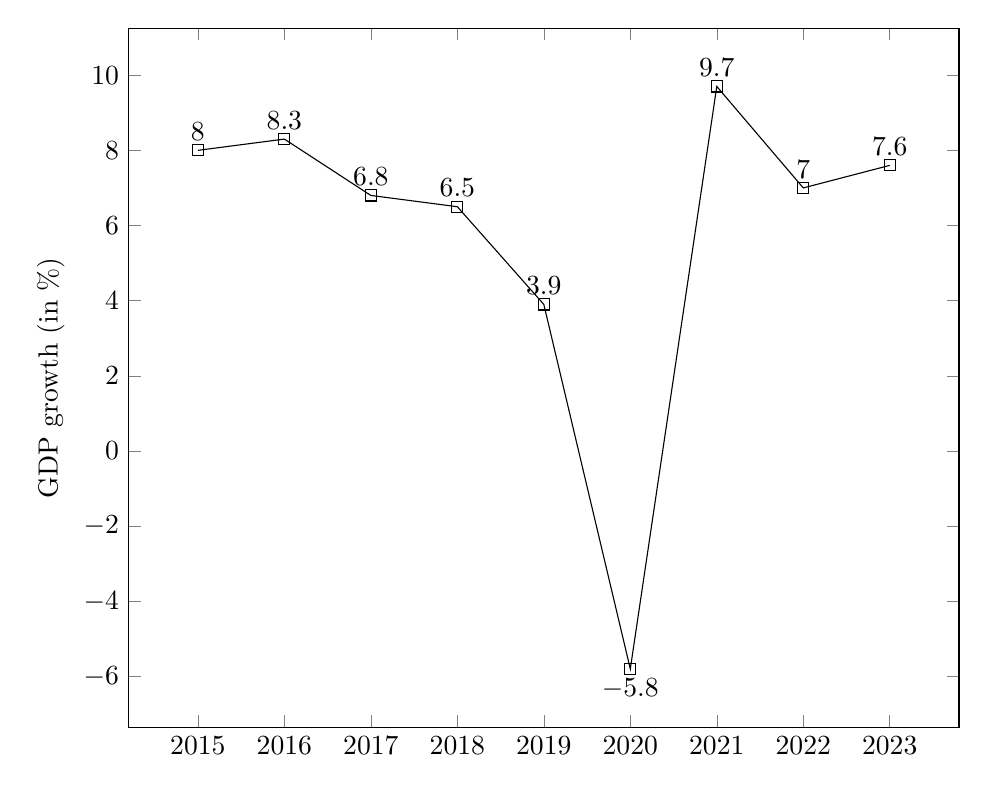
\begin{tikzpicture}
\begin{axis}[
xlabel={},
width=\textwidth,
mark=square,
ylabel={GDP growth (in \%)},
% remove comma in xticklabels
xticklabel style={/pgf/number format/set thousands separator={}},
xtick distance=1,
nodes near coords
]
\addplot[color=black, x={Year}, y={GDP growth (in \%)}] table {
2015 8
2016 8.3
2017 6.8
2018 6.5
2019 3.9
2020 -5.8
2021 9.7
2022 7
2023 7.6
};
\end{axis}
\end{tikzpicture}
\end{center}
\medskip
Source: World Bank
\smallskip
\hrule
\end{figure}

\section{Section Name}
\lipsum
\section{Conclusion}
\lipsum
\end{document}